\chapter{Statistics and Sampling Distributions}

\section{Statistics and Their Distributions}

Any sample mean can be regarded as a \textit{point estimate} of the population mean $\mu$.

\begin{definition}
    A \textbf{statistic} is any quantity whose value can be calculated from sample data. Prior to obtaining data, there is uncertainty as to what value of any particular statistic will result. Therefore, a statistic is a random variable and will be denoted by an uppercase letterl; a lowercase letter is used to represent the calculated or observed value of the statistic.
\end{definition}

\subsection{Random Samples}

\begin{definition}
    The rv's $X_1,\dots,X_n$ are said to form a (simple) \textbf{random sample} of size \textit{n} if 

    \begin{enumerate}
        \item The $X_i$'s are independent rv's.
        \item Every $X_i$ has the same probability distribution.
    \end{enumerate}

    Thus, $X_i$'s are \textbf{independent and identically distributed}(idd).

    The conditions are satisfied if sampling are with replacement, from an infinite population, or without replacement yet the sample size $n$ and population size $N$ satisfies $n/N\leq .05$(at most 5\% of the population is sampled).
\end{definition}

\section{The Distribution of the Sample Mean}

\begin{proposition}
    Let $X_1,\dots,X_n$ be a random sample from a distribution with mean value $\mu$ and standard deviation $\sigma$, then 

    \begin{enumerate}
        \item $E(\bar{X}) = \mu_{\bar{X}} = \mu$
        \item $V(\bar{X}) = \sigma_{\bar{X}}^2 = \sigma^2/n$ and $\sigma_{\bar{X}} = \sigma / \sqrt{n}$
        \item $E(T_o) = n\mu$
        \item $V(T_o) = n\sigma^2$ and $\sigma_{T_o} = \sqrt{n}\sigma$
    \end{enumerate}

    where $T_o = X_1 + \cdots + X_n$.
\end{proposition}

\subsection{The Case of a Normal Population Distribution}

\begin{proposition}
    Let $X_1,\dots,X_n$ be a random sample from a normal distribution with mean $\mu$ and stardard deviation $\sigma$. Then for any $n$, $\bar{X}$ is normally distributed(with mean $\mu$ and standard deviation $\sigma/\sqrt{n}$), as is $T_o$(with mean $n\mu$ and standard deviation $\sqrt{n}\sigma$).
\end{proposition}

\subsection{The Central Limit Theorem}

\begin{theorem}{THE CENTRAL LIMIT THEOREM(CLT)}
    Let $X_1,\dots,X_n$ be a random sample from a distribution with mean $\mu$ and variance $\sigma^2$. Then, in the limit as $n\rightarrow\infty$, the standardized versions of $\bar{X}$ and $T_o$ have the standard normal distribution. That is, 

    \begin{align*}
        \lim_{n\rightarrow\infty}P\left(\frac{\bar{X}-\mu}{\sigma/\sqrt{n}}\leq z\right) = P(Z\leq z)=\Phi(z) \\
    \end{align*}
    
    and 
    
    \begin{align*}
        \lim_{n\rightarrow\infty}P\left(\frac{T_o-n\mu}{\sqrt{n}\sigma/\sqrt{n}}\leq z\right) = P(Z\leq z)=\Phi(z) \\
    \end{align*}

    where $Z$ is a standard normal rv. $\bar{X}$ and $T_o$ are \textbf{asymptotically normal}.
\end{theorem}

Practical use of CLT: when $n$ is large and we wish to calculate a probability such as $P(a\leq \bar{X}\leq b)$, we need only to pretend that $\bar{X}$ is normal, standardize it and use the normal table. The resulting answer will be approximatedly correct, as shown in Figure \ref{fig:6-1}.

If $n>30$, the CLT can be used.

\begin{figure}[H]
    \centering
    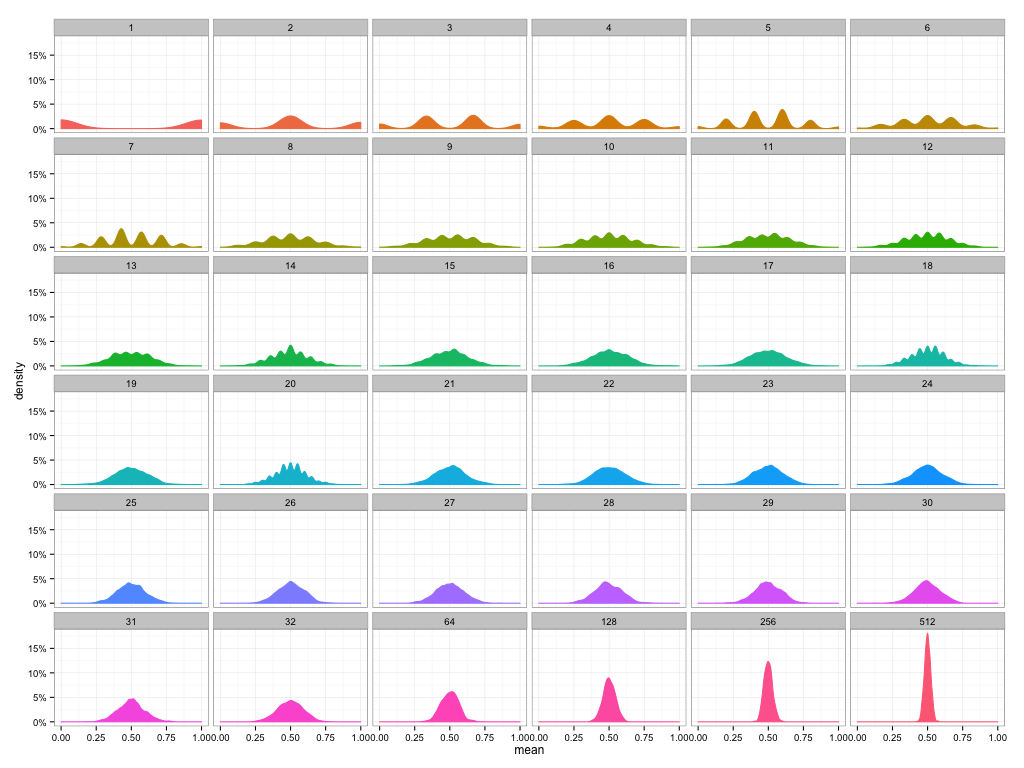
\includegraphics[width=0.9\textwidth]{img/6-central-limit-theorem.png}
    \caption{A simulation using the binomial distribution. Random 0s and 1s were generated, and then their means calculated for sample sizes ranging from 1 to 512. Note that as the sample size increases the tails become thinner and the distribution becomes more concentrated around the mean.(From Wikipedia.org)}
    \label{fig:6-1}
\end{figure}

\subsection{Other Applications of the Central Limit Theorem}

\begin{proposition}
    Let $X_1,\dots,X_n$ be a random sample from a distribution for which only positive values are possible($P(X_i > 0) = 1$). Then if $n$ is sufficiently large, the product $Y=X_1X_2\cdot\cdots\cdot X_n$ ahs approximately a lognormal distribution; that is, $\ln(Y)$ has a normal distribution.
\end{proposition}

\subsection{The Law of Large Number}

\begin{theorem}
    If $X_1,\dots,X_n$ is a random sample from a distribution with mean $\mu$ and variance $\sigma^2$, then $\bar{X}$ converges to $\mu$ 

    \begin{enumerate}[label=\textbf{\alph*.}]
        \item In mean square: \quad $E[(\bar{X}-\mu)]^2\rightarrow 0$ as $n\rightarrow \infty$
        \item In probability: \quad $P[|\bar{X} - \mu|\geq\epsilon\rightarrow 0]$ as $n\rightarrow 0$ for any $\epsilon > 0$
    \end{enumerate}
\end{theorem}

\section{The Mean, Variance, and MGF for Several Variables}

\begin{definition}
    Given a collection of $n$ rv's $X_1,\dots,X_n$ and $n$ numerical constants $a_1,\dots,a_n$, the rv 

    \begin{align*}
        Y=a_1X_1+\cdots+a_nX_n = \sum_{i=1}^na_iX_i \\
    \end{align*}

    is called a \textbf{linear combination} of the $X_i$'s.
\end{definition}

\begin{proposition}
    Let $X_1,\dots,X_n$ have mean values $\mu_1,\dots,\mu_n$ respectively, and variances $\sigma_1^2,\dots,\sigma_n^2$ respectively. 

    \begin{enumerate}
        \item Whether or not the $X_i$'s are independent, 
        
        \begin{align*}
            E(a_1X_1+\cdots+a_nX_n) & = a_1E(X_1) + \cdots + a_nE(X_n) \\
            & = a_1\mu_1 + \cdots + a_n\mu_n \\
        \end{align*}
        \item If $X_1,\dots,X_n$ are independent, 
        
        \begin{align*}
            V(a_1X_1 + \cdots + a_nX_n) & = a_1^2V(X_1) + \cdots + a_n^2V(X_n) \\
            & = a_1^2\sigma_1^2 + \cdots + a_n^2\sigma_n^2 \\
        \end{align*}

        and  

        \begin{align*}
            \sigma_{a_1X_1+\cdots+a_nX_n} = \sqrt{a_1^2\sigma_1^2 + \cdots + a_n^2\sigma_n^2} \\
        \end{align*}
        \item For any $X_1,\dots,X_n$, 
        
        \begin{align*}
            V(a_1X_1+\cdots+a_nX_n) = \sum_{i=1}^n\sum_{j=1}^na_ia_j\text{Cov}(X_i,X_j) \\
        \end{align*}
    \end{enumerate}
\end{proposition}

\subsection{The Difference Between Two Random Variables}

\begin{proposition}
    $E(X_1-X_2) = E(X_1) - E(X_2)$ and, if $X_1$ and $X_2$ are independent, $V(X_1-X_2) = V(X_1) + V(X_2)$.
\end{proposition}

\subsection{The Case of Normal Random Variables}

\begin{proposition}
    If $X_1,\dots,X_n$ are independent, normally distributed rv's, then any linear combination of the $X_i$'s also has a normal distribution. In particular, the difference $X_1 - X_2$ between two independent, normally distributed variables is itself normally distributed. 
\end{proposition}

\begin{proposition}
    Let $U$ and $V$ be linear combinations of the independent normal rv's $X_1,\dots,X_n$. Then the joint distribution of $U$ and $V$ is bivariate normal. The converse is also true. 
\end{proposition}

\subsection{Moment Generating Functions for Linear Combinations}

\begin{proposition}
    Let $X_1,\dots,X_n$ be independent rv's with moment generating functions $M_{X_1}(t),\dots,M_{X_n}(t)$, respectively. Define $Y=a_1X_1 + \cdots + a_nX_n$, where $a_1,\dots,a_n$ are constants. Then 

    \begin{align*}
        M_Y(t) = \prod_{k=1}^n M_{X_k}(a_kt) \\
    \end{align*}
    
    In the special case that $a_1=\cdots=a_n=1$, 
    
    \begin{align*}
        M_Y(t) = \prod_{k=1}^n M_{X_k}(t) \\
    \end{align*}

    which denotes the logarithm form of normal distribution convolution operations.
\end{proposition}

\section{Distributions Based on a Normal Random Sample}

Purpose: 

\begin{enumerate}
    \item Normal sample distribution is based on multiple normal rv's.
    \item Normal sample variance $\rightarrow$ normal rv's variance $\rightarrow$ distribution for sums of normal rv's squares $\rightarrow$ $\chi^2$ distribution
    \item Normal sample standard deviation $\rightarrow$ combine normal rv with square root of $\chi^2$ distribution $\rightarrow$ $t$ distribution
    \item Comparison of two normal sample variance $\rightarrow$ ratio of two $\chi^2$ distributions $\rightarrow$ $F$ distribution
\end{enumerate}

\subsection{The Chi-Squared Distribution}

Recall: $\chi^2$ distribution 

$\chi^2$ distribution is the special case of the gamma distribution with $\alpha=\upsilon/2$ and $\beta = 2$. 

The pdf of $\chi^2$ distribution is 

\begin{align*}
    f(x) = \left\{\begin{array}{cl}
        \frac{1}{2^{\upsilon/2}\Gamma(\upsilon/2)} x^{(\upsilon/2)-1} e^{-x/2} & x>0 \\
        0 & x\leq 0 \\
    \end{array}\right.
\end{align*}

where $\upsilon$ is degrees of freedom. 

The mean, variance and degrees of freedeom are 

\begin{align*}
    \mu = \alpha\beta = \upsilon \quad \sigma^2 = \alpha\beta^2 = 2\upsilon \quad M_X(t) = (1-2t)^{\upsilon/2} \\
\end{align*}

\begin{proposition}
    If $Z$ has a standard normal distribution and $X=Z^2$, then the pdf of $X$ is 

    \begin{align*}
        f(x) = \left\{\begin{array}{cl}
            \frac{1}{2^{1/2}\Gamma(1/2)} x^{(1/2)-1} e^{-x/2} & x > 0 \\
            0 & x\leq 0 \\
        \end{array}\right.
    \end{align*}

    $X$ is chi-squared with 1 df, or $X\sim \chi_1^2$.

    The conclusion can be derived by differentiating cdf of $X=Z^2$.
\end{proposition}

\begin{proposition}
    If $X_1\sim \chi_{\upsilon_1}^2$, $X_2\sim \chi_{\upsilon_2}^2$, and they are independent, then $X_1 + X_2 \sim \chi_{\upsilon_1 + \upsilon_2}^2$.

    The conclusion can be derived by MGF products.
\end{proposition}

\begin{proposition}
    The df of idd is add-ups of idd df's.

    If $Z_1,\dots,Z_n$ are independent standard normal distributions, then $Z_1^2 + \cdots + Z_n^2 \sim \chi_n^2$.
\end{proposition}

$\chi_{\alpha,\upsilon} = c$ means that $P(\chi_\upsilon^2 > c) = \alpha$(compared to $Z_\alpha = z\leftrightarrow P(Z\leq z) = \alpha$).

\begin{proposition}
    If $X_i$'s are a random sample from a normal distribution, then $\bar{X}$ and $S^2$ are independent.

    The conclusion can be derived by Covariance of the two items. 
\end{proposition}

\begin{proposition}
    If $X_3 = X_1 + X_2$, and $X_1\sim \chi_{\upsilon_1}^2$, $X_3\sim\chi_{\upsilon_3}^2$, $\upsilon_3>\upsilon_1$, and $X_1$ and $X_2$ are independent, then $X_2\sim \chi_{\upsilon_3 - \upsilon_1}^2$.

    The conclustion can be dirived by MGF products.
\end{proposition}

\begin{proposition}
    If $X_i$'s are a random sample from a normal distribution, then 
    
    \begin{align*}
        (n-1)S^2/\sigma^2\sim \chi_{n-1}^2 \\
    \end{align*}

    The df $n-1$ is based on the fact that for $X_i$, $s_i^2$ is based on the first $n-1$ $x_i$'s rather than all $x_i$'s.
\end{proposition}

\subsection{The $t$ Distribution}

\begin{theorem}
    If $X_1,\dots,X_n$ is a random sample from a normal distribution $N(\mu,\sigma^2)$, then variable has the $t$ distribution with $n-1$ df, $t_{n-1}$, is 

    \begin{align*}
        T=\frac{\bar{X}-\mu}{S/\sqrt{n}}=\frac{Z}{\sqrt{X/\upsilon}} \\
    \end{align*}

    The pdf of a rv $T$ with $t$ distribution and $\upsilon$ df is 

    \begin{align*}
        f(t) = \frac{1}{\sqrt{\pi}\upsilon}\frac{\Gamma[(\upsilon+1)/2]}{\Gamma(\upsilon/2)}\frac{1}{(1+t^2/\upsilon)^{(\upsilon+1)/2}}\quad -\infty<t<\infty
    \end{align*}

    The conclusion can be derived by differentiating the cdf of $t$ distribution.
\end{theorem}

\subsection{The $F$ Distribution}

\begin{definition}
    Let $X_1,X_2$ be independent $\chi^2$ rv's with $\upsilon_1$ and $\upsilon_2$ df. The $F$ distribution with $\upsilon_1$ numerator df and $\upsilon_2$ denominator df is 

    \begin{align*}
        F_{\upsilon_1,\upsilon_2}=\frac{X_1/\upsilon_1}{X_2/\upsilon_2} \\
    \end{align*}
\end{definition}
